\begin{student}
Hello and Welcome to your very first \textsc{PEN Education} \textbf{Mathematics} lesson! Today's topic shall be \underline{Whole Numbers}. But before we begin some context will serve you well:

Each week, you will receive a booklet typeset in this format\footnote{For those curious, the typesetting system is \LaTeX}, we have created approximately 150 such booklets for Math, and another 100 for English. The Mathematics booklets are based off the ICE-EM AMSI Cambridge Textbooks, written by tenured Professors of Mathematics who understand the content and the process of its Education well. If you are ever in the need for further study, or want clarification about a concept beyond what your tutor is able to provide - the textbook is always a fantastic thing to turn to.

Now, the structure of the booklets will always be as follows:
\begin{enumerate}
    \item An \textbf{introduction} to help contextualise the newly learned content with reference to what you have already learned\footnote{in the literature this effective learning principle is termed \emph{elaborative encoding}}
    \item Sectioned \textbf{topics} that each cover \emph{one} important concept. These topics will be listed in the \underline{Table of Contents} on the first page. Use this!
    \item Within each topic will be \textbf{Theory}\footnote{Note that you may not always have a theory section.}, \textbf{Examples} and \textbf{Exercises}
    \item Every question that requires an answer in these booklets will have a corresponding Mark allocated to it. The Marks are tallied in the GradeTable on the last page of every Booklet. Your tutor will mark your work every other week; if the work is not being done you/we should question your place in this tutoring centre. Your marks will be recorded for the statistical analysis.
    \item Each page now has margins inspired by \href{https://tug.ctan.org/macros/latex/contrib/tufte-latex/sample-book.pdf}{Edward Tufte}. Use them to flesh out new ideas as well as write out trivial sums you should know how to do.\reversemarginpar\marginpar{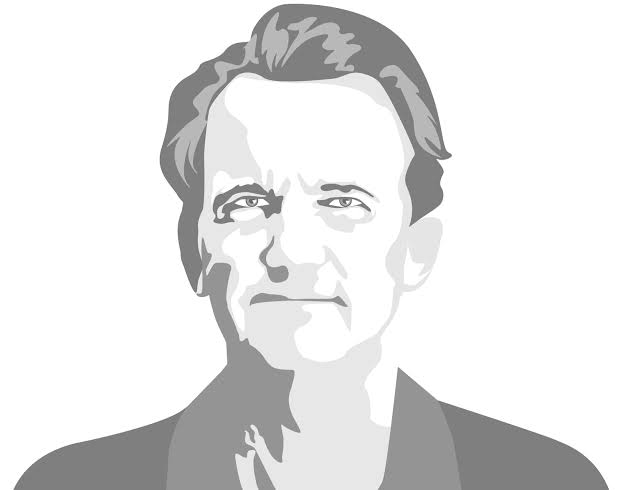
\includegraphics[width=1in]{tufte.jpg}}
    \item Homework:
\end{enumerate}

\subsection{Homework}
The concept of \emph{homework} is so important for us, that I am writing this in its own \emph{subsection}!\tikz[remember picture,overlay,baseline=0pt] \draw[->,thick,gray!50] (0.15,0.05) -- (0.15,1.15);



\smallskip
\fbox{
\fbox{
    \centering
\textsc{\small YOU MUST ATTEMPT ALL HOMEWORK THAT HAS BEEN PRESCRIBED TO YOU.}
}}
\smallskip

This is a law. It must be followed.

Note that, it is not compulsory to \textbf{always} do \textbf{all} of the Homework at the back of the booklet. The only thing that must be done, is the homework you have agreed to do.
It will often be the case that you have other assessment tasks to do. You might have an important Ochestra event to attend, you might have a family holiday planned. You might be sick, you might find it too difficult. All of these are valid --- speak to your tutor about it, they'll \emph{prescribe} you the appropriate amount of homework.

Furthermore, beyond the hurdles of everyday life that might 🛑STOP🛑 you from attempting homework, there is truly great benefit in sitting at home and thinking about the homework problems. You will gain further insight into the tiny little corners of the concepts you have learned. The homework problems have been designed to be slightly harder than the exercises, and the exercises in turn have been designed to be slightly harder than the example questions.

Finally, if you attempt the homework questions, you will be in a \emph{much} better position to score well in the Topic Tests.

\end{student}
\begin{instructor}
Hello and Welcome to the Circus. This Manual is for the instructor, and has been designed to be sparse.

    The pre-conditions for teaching this material is a Band 6 or equivalent in the NESA HSC Advanced Mathematics, and for the English booklets it will be a mid Band 5 and above. The post-conditions for this booklet, i.e. what it guarantees \emph{you}, is \textbf{answers} to all the \textsc{Example}, \textsc{Exercise} and \textsc{Homework Questions}. What it \underline{does not} guarantee you are solutions to the individual questions.

It is expected that you are able to solve all of these via your own volition. It is also expected that you designate homework each week. You may not necessarily be the one to mark it, but you must prescribe it.

    You will also notice that your copy significantly differs from that of the student---you are missing their theory. As a result, your pages numbers are entirely skewed and you should \textbf{not use} page numbers as a guide to find answers within this \textsc{Instructor's Manual}. Furthermore, it would benefit you to read this introduction section before teaching any and every class.

    Ideally, a utopic tutor will not need this \textsc{manual} beyond a cursory reading; s/he should hold a student copy of the booklet throughout class and read out loud the corresponding theory. It will also be of immense benefit for the tutor to delegate paragraphs for the students to read aloud. This will improve their engagement, understanding, reading-comprehension, pronunciation and classroom respect.

    \subsection{Aayush Bajaj}
    I will take a quick moment to introduce myself as my voice will propagate through these booklets. I am a $3^{\text{rd}}$ year Computer Science major at UNSW and went to a selective high school in Sydney. I understand the NESA syllabus well, but these booklets have been designed with the \emph{Australian} curriculum in mind.

    I have been teaching in classroom settings; primary school and high school as well as privately since I graduated in 2019. Since then I have consumed many books on meta-cognition, psychology and evidence-based learning---you will occasionally find references in the footnotes. Furthermore, I apply these to my own studies with great success.

    I typeset these booklets using \LaTeX, compiled with the LuaLatex engine under the \texttt{exam} class. The source code for both \textsc{Instructor} and \textsc{Student} copies lie in the same files and are distinguished by the boolean variable \texttt{printanswers}. For any interested \TeX\ nicians you may send me an email at j@abaj.io, but otherwise, the source code for this project is not available.

    Finally, in the way that Virgil was the guide of Dante Aligheiri---I too shall be your guide for this booklet series. I hope you learn things both from myself and your students, I am certainly learning much in producing these booklets por toi.

    Love,
    AJ
\end{instructor}
